\documentclass[11pt]{article}
\usepackage{graphicx}
\usepackage[margin=2.5cm]{geometry}
\usepackage{array}
\usepackage{tabu} 

\title{Project Proposal: Enhancing Social HRI using Affective Communication}
\author{Katie Winkle}

\begin{document}

\maketitle

\begin{abstract}

\end{abstract}

\section{Aims and Objectives}
\subsection{Aims}
The overall aim of this project is to investigate emotional expression in robot to human communication. Specifically of interest is the potential for robot to human emotion transfer and the potential benefits this might have. This can be expressed as two key project aims:

\begin{enumerate}
\item Investigate robot to human emotion transfer
\item Investigate the impact of affective robot communication
\end{enumerate}

The first aim deals specifically with exploring emotion transfer, i.e. whether a human's emotional state can be changed through interaction with an emotionally expressive robot. The second aim is to demonstrate, regardless of whether emotion transfer occurs, how such emotional expression might impact on human-robot interaction (HRI). Some aspects for consideration are listed under Objective 3 however defining specific evaluation measures is non-trivial and makes up part of the required investigation. Generally it is the impact on the robot's effectiveness that should be considered; however the definition of effectiveness depends on the purpose of the robot. 

\subsection{Objectives}
In order to achieve the project aims, a list of specific objectives has been derived as follows: 
\begin{enumerate}
\item Study affective communication and emotion contagion
\item Create a parameterised model for generating emotional robot expression
\begin{itemize}
\item Conduct a model evaluation experiment for refinement
\end{itemize}
\item Conduct HRI experiment(s) to test the effects of affective robot communication
\begin{itemize}
\item Consider human/robot task performance and human emotional state
\end{itemize}
\end{enumerate}

\section{Motivation}
The psychological phenomenon of interpersonal emotion transfer (IET) between humans is still not fully understood; however it is believed to include social appraisal and emotion contagion effects \cite{parkinson2011interpersonal}. In this context social appraisal describes a person's judgement of something being affected by the emotional response of another (i.e. affecting what they think), whereas emotion contagion describes a change in their emotional state (i.e. affecting how they feel). For example, it has been demonstrated that listening to a neutral text spoken happily or sadly can induce similar feelings in the listener \cite{neumann2000mood} and that the same household object will be rated differently if it is presented alongside a picture of a smiling or disgusted face \cite{bayliss2007affective}. In addition, there is growing evidence that nonverbal emotional expression is an important and subconscious part of human communication which has evolved as a mechanism for quickly communicating a range of information such as social status and level of threat (see \cite{tracy2015nonverbal} for a review). 

Based on this there are at least two major reasons for wanting to design a robot with IET capabilities. Firstly, if emotional expression is an important part of human communication, then a robot with such capabilities might be more lifelike, more likeable and more natural to interact with. Secondly, the effects of IET described above, e.g shaping people's judgement or decision making and impacting on how they feel might be beneficial in a range of HRI applications just as it is in human-human interaction (HHI). In fact, example HRI scenarios where emotional expression might be useful might follow directly from those we can imagine in HHI, e.g. in encouraging children or care of the unwell; applications for which social robots have already been demonstrated (e.g. \cite{shiomi2015can}, \cite{gockley2006encouraging}). As one speculative example, endowing an social assisted living robot with IET  capabilities might offer the following functionality benefits: 
\begin{itemize}
\item the robot could provide more realistic and enjoyable social companionship
\item the robot could `cheer up' the user by being cheerful itself
\item the robot could give the user a positive impression of potentially undesirable tasks, e.g. taking medication or doing exercise
\item the robot could provide more effective encouragement during activities like those above
\item the robot could appear empathetic and caring, leading to a better human-robot relationship
\end{itemize}

However, this reasoning assumes that IET occurs equally well in HRI as HHI and that the effects on the human partner would be the same as if it was a human rather than a robot they were interacting with. Arguably, given the well known effect of the `uncanny valley'[REFERENCE?]; this assumption might not be valid and hence warrants further study. Research done so far suggest demonstrates that recognisable emotional expression is certainly possible in a range of robots (e.g. X X X from lit review), however the impact of this on a human's own emotional state and the robot's effectiveness is less well documented. 

In summary, the potential benefits of robot emotional expression and robot to human IET are clear. However, there is still significant uncertainty and a lack of evidence surrounding whether IET from a robot to a human can occur  and, if so, what impact this might have on the robot's effectiveness and/or the human's task performance. Addressing this uncertainty and lack of evidence in order to evaluate the real-world potential of robot-human IET forms the main motivation for undertaking this project. 

\section{Literature Review}
\subsection{IET and Emotional Expression in Humans}
There are different hypotheses concerning the purpose of IET and emotional expression more generally in HHI. A functionalist approach (considering the consequences in order to determine the purpose) suggests that at the dyadic level, emotion expressions help individuals determine other's emotions, beliefs, intentions and orientation towards their relationship (i.e. dominant or submissive); and that evoking emotions in others is associated with behaviours such as avoidance, helping, affiliation and soothing \cite{keltner1999social}. An evolutionary approach (considering development over time and the link to population fitness) suggests that emotional expression evolved from being a physiological response (e.g. scrunching the nose to prevent inhalation of noxious gas) into a form of social communication, which observers evolved an ability to instantly and subconsciously decode in order to obtain information about the expresser and/or their environment \cite{shariff2011emotion}. One consistent theme in the psychology literature however is the importance and subconscious nature of IET resulting from emotional expression in communication, and this is what has the most potential for use in HRI. 

There is evidence to suggest that one form of IET is social appraisal, whereby individual human judgement is influenced the perceived judgement of others \cite{parkinson2011interpersonal}. Specifically it has been demonstrated that judgement of an everyday object is different depending on whether it is presented alongside a smiling or disgusted face \cite{bayliss2007affective} which suggests that emotional expression is a trigger for this form of IET. Another experiment demonstrated that even in a very dangerous situation (a simulated fire) participants surrounded by seemingly calm and unresponsive actors were slower to react than participants that were alone; it has been argued that this could be due to IET effects whereby the participants felt calmer due to the calmness of the actors and also judged the situation to be less dangerous based on their percieved lack of concern (\cite{latane1968group} as discussed in \cite{parkinson2011interpersonal}).

Another evidenced form of IET is emotion contagion, whereby an individual's emotional state changes to based on that of their interaction partner; however this is less well understood and more difficult to experimentally examine than social appraisal effects \cite{parkinson2011interpersonal}. There is a general consensus that most emotion contagion is a form of social mimicry, however it is disputed whether this is based on physical mimicry in which the related emotion is generated from mimicking the physical expression; i.e. the individual smiles in response to a smile and hence feels happier \cite{strack1988inhibiting}, or whether expression is less important and actually an individual must understand and perceive the reason for another's emotional expression in order for emotion contagion to occur \cite{tamietto2009unseen}. In contrast to the idea of simple mimicry however it should also be noted that emotion contagion has been demonstrated to induce contrasting rather than matching emotions, and that this may be linked to social stature \cite{tiedens2003power}.

Demonstrated examples of emotion contagion highlight the impact it can have both at the individual and group level. For example, listening to neutral information spoken in an emotional way can induce similar emotions in the listener \cite{neumann2000mood}, and emotion contagion in a group can improve attitudes and reduce conflicts resulting in improved task performance \cite{barsade2002ripple}. It has even been demonstrated that emotion contagion can occur through social networks with Facebook users producing more positive or negative posts when the amount of negative or positive emotional content in their newsfeed was reduced \cite{kramer2014experimental} respectively. Other interesting results include thirsty individuals pouring more or less from a drink jug if exposed to a smiling or frowning face respectively \cite{winkielman2005unconscious} or acceptance of an offer being higher for smiling and lower for frowning proposers compared to those that wore neutral expressions \cite{mussel2013value}. 

In summary there is clear evidence that, whilst the origins and exact mechanisms of IET are not clear, it has significant impact on HHI and can influence an individual's feelings, judgement and behaviour as well as group collaboration and effectiveness. This surely warrants the study of IET in HRI in order to establish whether the same effects can be observed, and if so whether they can be useful e.g. in improving robot design (trying to say how much people like them?) or in improving task performance. Key research questions are whether robot to human IET can occur and how robot emotional expressions affect humans' judgements and behaviour. Additionally the ability to experiment with individual elements of emotional expression in a controlled way, as possible on a robotic platform, might be useful in demonstrating and contributing to some of the theories on IET in the psychology literature. 

In order to design emotionally expressive robot behaviours it must first be established how emotion is expressed in humans and identify specific behaviours which might be transferable onto a robot. Specifically the robotic platform to be used for this project is Aldebaran Robotics' humanoid robot
NAO [REFERENCE OR FOOTNOTE MAYBE?], which means that facial expression cannot be altered and hence lies outside the scope of this project. It is noted that facial expression forms an important part of affective communication [REFERENCE] and so further work in the future would be to extend the investigation proposed here to include that. However, it has been demonstrated that regardless of facial expression or a lack thereof, emotion can be recognised from voice and movement alone [REFERENCES] and previous demonstrations of emotional behaviour implemented on the NAO suggest it is certainly possible... [Lim, Xu etc]. 

The study of emotion recognition in point light displays generated from emotional dance and acting performances has demonstrated that movement alone can express emotion even if the semantic purpose of that movement is unknown (e.g. \cite{dittrich1996perception}, \cite{pollick2001perceiving}, \cite{atkinson2004emotion}). Laban Movement Analysis (LMA), a multidisciplinary tool for movement analysis considering parameters such as weight, space and time, has become a standard method for parameterising movement in order to further study such effects \cite{lab2011}. As such, instructions on how to perform a certain emotion, as might be explained to dancers or actors, typically utilise LMA [REFERENCE]. Similarly it is widely accepted that emotion can be portrayed through neutral speech or across languages [REFERENCES] and similar to LMA, this can be quantitatively described by variation in parameters such as XXX [REFERENCES]. One important conclusion from these findings is that emotion can theoretically be expressed through any movement or speech, regardless of semantic content. This is particularly relevant for robotiscists because it means that emotional expression can be added to communication or task execution without changing the robot's functional behaviour. [something about therefore idea of using parameterised model is good? or highlights where to look to figure out which parameters to set]

This principle (has been/is) commonly used in animation...[some cool animation reference to Pixar Lamp or Disney or something - this might be better in with the Laban movement stuff]. This is an important result for robotics because it demonstrates that a lack of facial expression capabilities does not render a robot incapable of emotional expression. In addition, the idea that the semantics of a gesture are not necessarily related to the emotion it might express is important for robotiscists who wish to endow their robots with emotional expression capabilities without impacting on their functional behaviour. 

Given this concept of semantic free emotional expression via motion, an obvious question then becomes what are the parameters and variables that determine the emotional content of movement? One well-respected method for parameterising human body movement is Laban Movement Analysis (LMA);. This has been used directly in robot emotion generation (e.g \cite{masuda2010motion}) as well as providing inspiration generally for the use of parameterised frameworks in emotional motion generation (e.g. \cite{lim2011converting}, \cite{xu2013mood}). These models are discussed further in the following section. -> instead start next section with 'these models were inspired by or use LMA...'

KEY FINDINGS/RELEVANCE/RESEARCH QUESTIONS

\subsection{Emotional Expression, IET in Robots \& Affective (or related?) HRI Studies}

**May want to use related rather than affective in title if want to reference related but not affective studies e.g. touching on motivation, persuasion. Or could have an entire section on evaluation methodologies discussing example experimental setups and what they measured etc. 

[Voice - something about emotional voice generation easily do-able using speech generation tools, maybe a robot example that uses specific tool I want to use - see meeting notes. Need to at least talk about proposed method(s) of voice generation; said tool or actor samples]

Masuda and Koto's system uses ths in a speech sample. Implemented on a NAO the resulting motion had an emotion recognition rate of above 60\% and, when combined with the original speech sample, lead to improved recognition rates fe six main parameters of LMA: space, time, weight, inclination, height and area, which are set based on previous analysis of observed movement emotion classification from a pilot experiment \cite{masuda2009emotion}. Implemented on a humanoid robot the resulting motion had an average emotion recognition rate greater than 60\% \cite{masuda2010motion}. Lim et al.'s framework for adding emotion to gesturing uses four parameters: speed, intensity, regularity and extent, which are set based on a mapping from the same featureor the emotions of happiness and sadness compared to speech alone \cite{lim2011converting}. Xu et al.'s framework uses a combination of general motion and pose parameters (e.g. speed, decay rate, stroke curves) as well as gesture specific ones (e.g. palm up or down). In addition the head is utilised as an effector which can be set in different poses. Parameter settings were then derived by averaging the results of an experiment in which participants were asked to set them in order to achieve specific emotional expressions on a NAO \cite{xu2013mood}. A later experiment demonstrated that different arousal and valence states can be recognised based on these parameters however no results for specific emotion recognition were described \cite{xu2013bodily}.

In the field of socially assistive robotics, there is evidence that robotoscists are already utilising such techniques with some reported success, although this is limited and generally based on qualitative data. For example, Fasola and Matari{\'c} presented a robot exercise coach for the elderly which they claimed participants enjoyed working with and hence were more likely to complete their exercise, however no quantitative data was recorded \cite{fasola2010robot} MAYBE REPLACE WITH ANOTHER SPECIFIC EMOTION-RELATED EXAMPLE. Tielman et al. demonstrated an adaptive emotion model implemented on a NAO used to play a quiz game with children; by using questionnaires they determined that children found emotional expression to be a positive trait for a robot but again no quantitative date was recorded \cite{tielman2014adaptive}. Even in a long term study documenting the use of a humanoid game playing robot in an elderly care home, which did quantify how emotional expression ranked as a positive trait compared to other characteristics through surveying, collected no data on task performance or interaction rates \cite{louie2012playing}. Such results highlight the lack of clarity and evidence available as to the true effect of emotional expression, including whether robot to human IET can occur, however it does highlight that...maybe something about no comparisons to non-emotional robot etc...some measure of how well liked the robot is or how much the emotional expression adds to the enjoyment of using the robot is in itself a form of effectiveness, and this should be taken into account when designing measurement criteria for the experiment undertaken in this project. This is noted under the third project objective which lists 'robot task performance' of one of the potential criteria for measuring experimentally; if one of the tasks of the robot is to be a pleasant companion and emotional expression is given as something particularly liked about the robot then arguably the emotional expression has improved the robot's task performance.  

There are other studies in the field of SAR and more general HRI however which, whilst generally looking at the impact of the overall robot rather than a specific trait such as emotional expression, demonstrate quantitative experimental data collection and are hence useful to consider and take inspiration from in the experimental design for this project...weight loss robot, science curiosity?, sign language tutoring, encouraging therapy, robot touch on task performance, designing persuasive robot...

[Second Xu paper on actual emotion contagion results as only example found to bring all above together, highlight how they measured etc and what i will do same/different/better]


KEY FINDINGS/RELEVANCE/RESEARCH QUESTIONS

An objective of this project is to create a such a framework, and hence studying which parameters these models utilise, how those parameters are set and experimental results for emotion recognition is a worthwhile exercise.

[conclusion for model design - Lim easy and similar results, Xu may not generalise so well but use of head could increase recognition rates, interesting idea of crowdsourcing as way to get parameters etc... Given that using voice too Lim's model might make most sense but will it work so well with a speech generator input as human speech samples?]

***************Paul's Notes***************

For the literature review I would break it up in to several sections:

IET and emotional expressions in humans. While there is some on this already in the motivation section I think it would be good to have more detail to frame what you are proposing to do with the robot.

Emotional expression in robots and HRI studies using an affective component. You might also consider the animated agent literature (sometimes called embodied communication agents).

IET in robots/animated agents

For each piece/area of research you should aim to summarise the key findings and how it is of relevance to your work. This could be identifying things wrong/missing from the literature, or how your work is using previous findings to inform what you are doing. These relating of the literature to your work could be from individual pieces, or an area of several pieces, whatever makes the most sense. You will also likely want a conclusion to you review that tries to tie the various sections together and how they are resulting in research questions.

*****************************************************

\subsection{Experimentally Evaluating Affective Impact}

\section{Risk Register}
%\begin{tabu} to \textwidth { | X[l] | X[l] | X[c] | X[c] | X[c] | }
%\begin{tabular}{|c|c|c|c|c|}
\begin{center}
	\begin{tabular}{|m{6cm}|m{5cm}|m{1.8cm}|m{1cm}|m{1cm}|}
		\hline
		Risk & Mitigation & Likelihood & Impact & \textbf{Score} \\
		\hline
		Emotion generation model not ready in time for final experiment & Hand script behaviours to allow experiment to go ahead & 2 & 3 & \textbf{6} \\ 
		\hline
		Identified emotional behaviours from literature do not transfer onto robot platform & Identify many alternative behaviours and form a prioritised list to work through and test, consider the most 'simple' emotions first & 2 & 4 & \textbf{8} \\ 
		\hline 
		Issue with hardware of robot platform preventing experiment being undertaken & Some time in plan for rescheduling, or could implement reduced experiment using virtual agent & 2 & 3 & \textbf{6} \\
		\hline 
		Cannot recruit enough participants for statistical significance in experiment(s) & Start recruiting in sensible advance of experiment, use within rather than between subject experiment design, consider virtual alternatives such as video surveys & 3 & 3 & \textbf{9} \\
		\hline
	\end{tabular} 
\end{center}
%\end{tabu}

\section{Timeline}
A Gantt Chart showing key project activities and their suggested time allocations is given in Figure \ref{fig:ProjectTimeline}. 

\begin{figure}
\centering
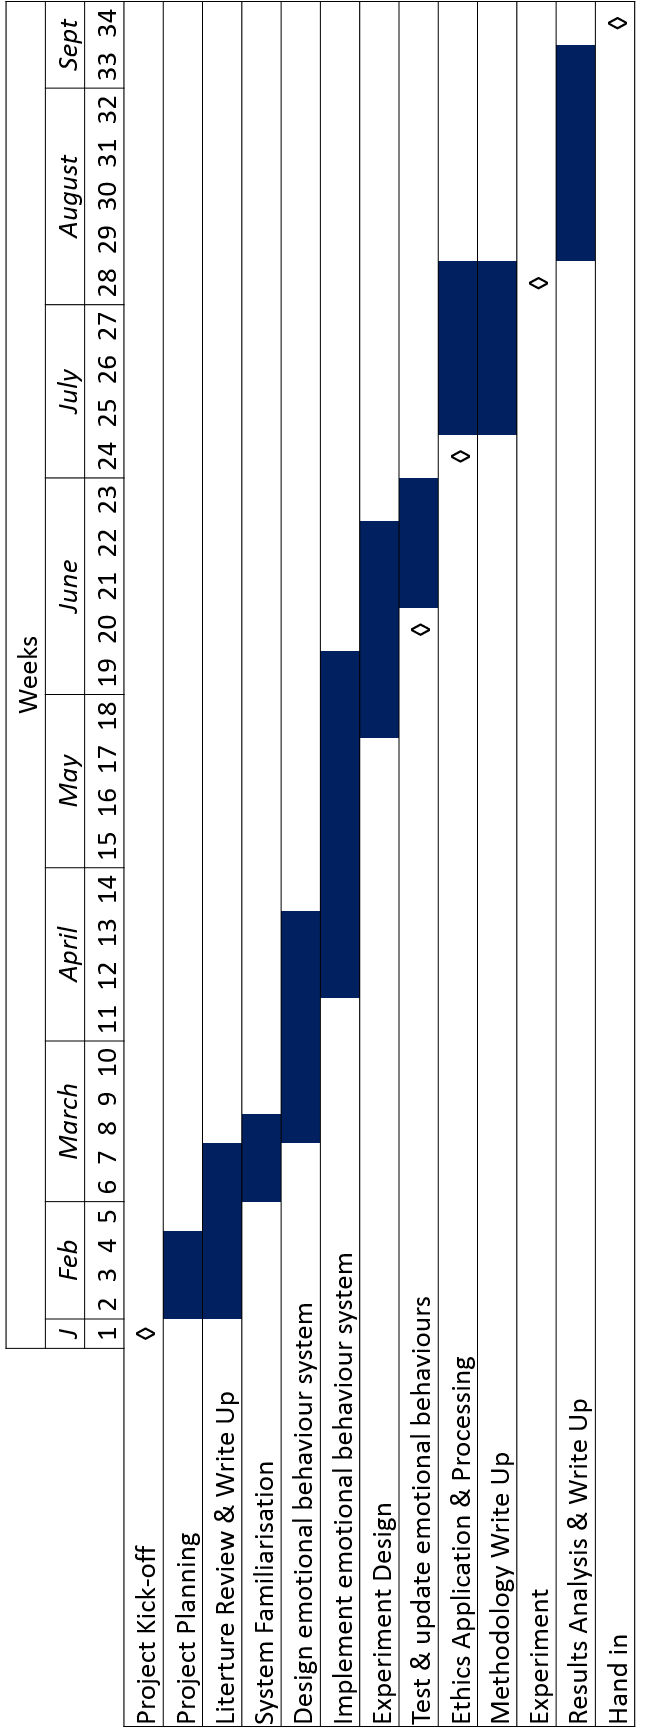
\includegraphics[height=0.9\textheight,]{ProjectTimeline2.png}
\caption{Project timeline - diamonds indicate discrete timing point events.}
\label{fig:ProjectTimeline}
\end{figure}

\bibliographystyle{unsrt}
\bibliography{ProjectReferences}
\end{document}
